%iffalse
\let\negmedspace\undefined
\let\negthickspace\undefined
\documentclass[journal,12pt,onecolumn]{IEEEtran}
\usepackage{cite}
\usepackage{amsmath,amssymb,amsfonts,amsthm}
\usepackage{algorithmic}
\usepackage{multicol}
\usepackage{circuitikz}
\usepackage{tikz}
\usepackage{graphicx}
\usepackage{textcomp}
\usepackage{xcolor}
\usepackage{txfonts}
\usepackage{listings}
\usepackage{enumitem}
\usepackage{mathtools}
\usepackage{gensymb}
\usepackage{comment}
\usepackage[breaklinks=true]{hyperref}
\usepackage{tkz-euclide} 
\usepackage{listings}
\usepackage{gvv} 
\usepackage{tikz}
\usetikzlibrary{shapes,arrows} 

%\def\inputGnumericTable{}                                
\usepackage[latin1]{inputenc}                                
\usepackage{color}                                            
\usepackage{array}                                            
\usepackage{longtable}                                       
\usepackage{calc}                                             
\usepackage{multirow}                                         
\usepackage{hhline}                                           
\usepackage{ifthen}                                           
\usepackage{lscape}
\usepackage{tabularx}
\usepackage{array}
\usepackage{float}
\newtheorem{theorem}{Theorem}[section]
\newtheorem{problem}{Problem}
\newtheorem{proposition}{Proposition}[section]
\newtheorem{lemma}{Lemma}[section]
\newtheorem{corollary}[theorem]{Corollary}
\newtheorem{example}{Example}[section]
\newtheorem{definition}[problem]{Definition}
\newcommand{\BEQA}{\begin{eqnarray}}
\newcommand{\EEQA}{\end{eqnarray}}
\newcommand{\define}{\stackrel{\triangle}{=}}
\theoremstyle{remark}


% Marks the beginning of the document
\begin{document}
\bibliographystyle{IEEEtran}
\vspace{3cm}

\title{\textbf{2007-EE-35-51}}
\author{AI24BTEC11027 - R Sumanth}
\maketitle
\bigskip

\renewcommand{\thefigure}{\theenumi}
\renewcommand{\thetable}{\theenumi}
\setlength{\columnsep}{2.5em}
\begin{enumerate}
    

\item The system $\frac{900}{s(s+1)(s+9)}$ is to be compensated such that its gain-crossover frequency becomes same as its uncompensated phase-crossover frequency and provides a $45 \degree$ phase margin. To achieve this, one may use 
\begin{enumerate}
    \item a lag compensator that provides an attenuation of $20$ dB and a phase lag of $45\degree$ at the frequency of $3\sqrt{3}$ rad/s
    \item a lead compensator that provides an amplification of $20$ dB and a phase lead of $45 \degree$ at the frequency of $3$ rad/s.
    \item a lag-lead compensator that provides an amplification of $20$ dB and a phase lag of $45 \degree$ at the frequency of $\sqrt{3}$ rad/s.
    \item a lag-lead compensator that provides an attenuation of $20$ dB and phase lead of $45 \degree$ at the frequency of $3$ rad/s.\\
\end{enumerate} 

\item Consider the discrete-time system shown in the figure where the impulse response of G(z) is $g(0)=0, g(1)=g(2)=1, g(3)=g(4)=...=0.$ \\

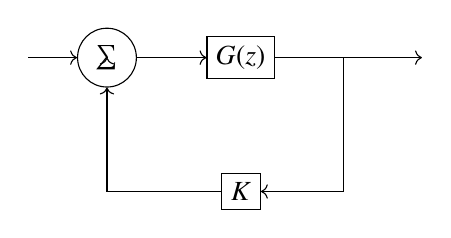
\begin{tikzpicture}[node distance=1.7cm] \node[circle, draw] (sum) {$\sum$}; \node[rectangle, draw, right of=sum] (Gp) {$G(z)$}; \node[rectangle, draw, below of=Gp] (K) {$K$};
\draw[->] (-1,0) -- (sum);
\draw[->] (sum) -- (Gp);  \draw[->] (K) -| (sum); \draw[->] (0,0) -- (sum); \draw[->] (Gp) -- (4,0);
\draw[->] (3,0) |- (K);
\end{tikzpicture}

 This system is stable for range of values of $K$ 
 
\begin{enumerate}
\item $[-1, \frac{1}{2}]$
\item $[-1, 1]$
\item $[\frac{-1}{2}, 1]$
\item $[\frac{-1}{2}, 2]$\\
\end{enumerate} 

\item A signal $x(t)$ is given by \\
$ x(t) = \begin{cases} 
1, & -\frac{T}{4} < t \leq \frac{3T}{4} \\
-1, & \frac{3T}{4} < t \leq \frac{7T}{4} \\
-x(t+T) 
\end{cases} $ \\

Which among the following gives the fundamental fourier term of $x(t)$? 
\begin{enumerate}
\item $\frac{4}{\pi} \cos{\frac{\pi t}{T}-\frac{\pi}{4}}$
\item $\frac{\pi}{4} \cos{\frac{\pi t}{2T}+\frac{\pi}{4}}$
\item $\frac{4}{\pi} \sin{\frac{\pi t}{2T}-\frac{\pi}{4}}$
\item $\frac{\pi}{4} \cos{\frac{\pi t}{2T}+\frac{\pi}{4}}$ \\
\end{enumerate}

\item If the loop gain $K$ of a negative feedback system having a loop transfer function $\frac{K(s+3)}{(s+8)^2}$ is to be adjusted to induce a sustained oscillation then 
\begin{enumerate}
\item The frequency of this oscillation must be $\frac{4}{\sqrt{3}}$ rad/s
\item The frequency os this oscillation must be must be 4 rad/s
\item The frequency of this oscillation must be must be 4 or $\frac{4}{\sqrt{3}}$ rad/s
\item such a $k$ does not exist \\
\end{enumerate}

\item The system shown in figure below 

\begin{figure}[!ht]
\centering
\resizebox{0.7\textwidth}{!}{%
\begin{circuitikz}
\tikzstyle{every node}=[font=\LARGE]

% Top horizontal line
\draw (0,10.75) to[short] (12.75,10.75);
\draw [->, >=Stealth] (12.75,10.75) -- (12.75,9.25);
\draw [->, >=Stealth] (4.25,10.75) -- (4.25,9.25);

% Rectangles and labels
\draw  (3,9.25) rectangle (5.5,8);
\draw  (11.5,9.25) rectangle (14,8);
\draw  (7.25,9.25) rectangle (9.75,8);
\draw  (1.25,9.25) rectangle (-1.25,8);
\draw (0,10.75) to[short] (-2,10.75);
\draw (-2.25,9.75) to[short] (-2.25,1.5);

% More lines and feedback loops
\draw [->, >=Stealth] (8.5,9.75) -- (8.5,9.25);
\draw [->, >=Stealth] (0,9.75) -- (0,9.25);
\draw  (10.75,6.25) circle (1cm);
\draw (8.5,8) to[short] (8.5,6.25);
\draw (12.75,8) to[short] (12.75,6.25);
\draw [->, >=Stealth] (8.5,6.25) -- (9.75,6.25);
\draw [->, >=Stealth] (12.75,6.25) -- (11.75,6.25);

% More circles and lines
\draw [->, >=Stealth] (10.75,5.25) -- (10.75,4);
\draw  (10.75,3) circle (1cm);
\draw  (2,3) circle (1cm);
\draw (4.25,8) to[short] (4.25,4.5);
\draw (4.25,4.5) to[short] (2,4.5);
\draw (0,8) to[short] (0,3);
\draw [->, >=Stealth] (0,3) -- (1,3);
\draw [->, >=Stealth] (2,4.5) -- (2,4);
\draw  (5,3.75) rectangle (7.75,2.5);
\draw [->, >=Stealth] (3,3) -- (5,3);
\draw [->, >=Stealth] (7.75,3) -- (9.75,3);
\draw [->, >=Stealth] (11.75,3) -- (13.5,3);
\draw  (13.5,3.75) rectangle (16.5,2.5);
\draw [->, >=Stealth] (16.5,3) -- (18,3);
\draw  (18,3.75) rectangle (21,2.5);
\draw [->, >=Stealth] (21,3) -- (22.75,3);

% Bottom rectangles and lines
\draw  (0.5,1) rectangle (3.5,-0.25);
\draw  (9.5,1) rectangle (12.5,-0.25);
\draw (-2.25,1.5) to[short] (-2.25,-1.75);
\draw (-2.25,-1.75) to[short] (15,-1.75);
\draw (15,-1.75) to[short] (22,-1.75);
\draw (22,-1.75) to[short] (22,3);
\draw (17.25,3) to[short] (17.25,-1);
\draw (17.25,-1) to[short] (2,-1);
\draw [->, >=Stealth] (2,-1) -- (2,-0.25);
\draw [->, >=Stealth] (11,-1) -- (11,-0.25);

% Node Labels
\node [font=\Large] at (0,8.5) {$b_0$};
\node [font=\Large] at (4.25,8.5) {$c_0$};
\node [font=\Large] at (8.5,8.5) {$b_1$};
\node [font=\Large] at (12.75,8.5) {$c_1$};
\node [font=\Large] at (10.75,3) {$\sum$};
\node [font=\Large] at (15,3) {1/s};
\node [font=\Large] at (6.25,3) {1/s};
\node [font=\Large] at (2,3) {$\sum$};
\node [font=\Large] at (19.5,3) {$P$};
\node [font=\Large] at (2,0.5) {$a_0$};
\node [font=\Large] at (11,0.5) {$a_1$};
\node [font=\Large] at (10.75,6.25) {$\sum$};

% Summation and +/- signs
\node [font=\Large] at (1,4) {+};
\node [font=\Large] at (12.25,5.75) {+};
\node [font=\Large] at (11.75,4) {+};
\node [font=\Large] at (9.25,7) {+};
\node [font=\Large] at (2.5,4.25) {+};
\node [font=\Large] at (9.5,3.75) {+};
\node [font=\Large] at (0.75,2.5) {-};
\node [font=\Large] at (9.75,2) {-};

% Bottom circles and lines
\draw [->, >=Stealth] (10.75,1) -- (10.75,2);
\draw (-2.25,9.75) to[short] (3.75,9.75);
\draw (4.75,9.75) to[short] (8.5,9.75);
\draw (3.75,9.75) to[short] (4.75,9.75);

\end{circuitikz}
}%

\label{fig:my_label}
\end{figure}

can be reduced to the form

\begin{figure}[!ht]
\centering
\resizebox{0.5\textwidth}{!}{%
\begin{circuitikz}
\tikzstyle{every node}=[font=\LARGE]
\draw [->, >=Stealth] (0.5,7.25) -- (1.5,7.25);
\draw  (1.5,8) rectangle (4,6.5);
\draw [->, >=Stealth] (4,7.25) -- (5,7.25);
\draw  (7.5,8) rectangle (10,6.5);
\draw  (5.75,7.25) circle (0.75cm);
\draw [->, >=Stealth] (6.5,7.25) -- (7.5,7.25);
\draw [->, >=Stealth] (10,7.25) -- (11,7.25);
\draw  (11,8) rectangle (13.5,6.5);
\draw [->, >=Stealth] (13.5,7.25) -- (14.5,7.25);
\draw (14,7.25) to[short] (14,5.5);
\draw (14,5.5) to[short] (14,5);
\draw  (10,5.75) rectangle (7.5,4.25);
\draw [->, >=Stealth] (14,5) -- (10,5);
\draw (7.5,5) to[short] (5.75,5);
\draw [->, >=Stealth] (5.75,5) -- (5.75,6.5);
\node [font=\LARGE] at (2.75,7.25) {X};
\node [font=\LARGE] at (5.75,7.25) {$\sum$};
\node [font=\LARGE] at (8.75,7.25) {Y};
\node [font=\LARGE] at (12.25,7.25) {P};
\node [font=\LARGE] at (8.75,5) {Z};
\node [font=\LARGE] at (5.25,6.25) {+};
\node [font=\LARGE] at (4.75,7.75) {+};
\end{circuitikz}
}%

\label{fig:my_label}
\end{figure}

with

\begin{enumerate}
    \item $X=c_0s+c_1, Y=\frac{1}{(s^2+a_0s+a_1)}' Z=b_0+b_1$
    \item $X=1, Y=\frac{1}{(s^2+a_0s+a_1)} 'Z=b_0s+b_1$
    \item $X=c_1s+c_0, Y=\frac{(b_1s+b_0)}{(s^2+a_1s+a_0)}'Z=1$
    \item $X=c_1+c_0,Y=\frac{1}{(s^2+a_1s+a_0)}'Z=b_1s+b_0$\\
\end{enumerate}

\item The value $\oint_c \frac{dz}{(1+z^2)}$ where C is the contour $|z-\frac{i}{2}|=1$ is 
\begin{enumerate}
    \item $2\pi i$
    \item $\pi$
    \item $\tan^{-1}x$
    \item $\pi i \tan^{-1}z$\\
\end{enumerate}

\item A single-phase voltage source inverter is controlled in a single pluse-width modulated mode with a pluse width of $150\degree$ in each half cycle. total harmonic distortion is defined as THD=$\frac{\sqrt{V_{rms}^2-V_1^2}}{V_1}\times 100$, where $V_1$ is the rms value of the fundamental component of the output voltage. the THD of output ac voltage waveform is 
\begin{enumerate}
    \item $65.65\% $
    \item $48.42\%$
    \item $31.83\% $
    \item $30.49 \%$\\
\end{enumerate}

\item A voltage source inverter is used to control the speed of a three-phase,$50 Hz$, squirrel cage induction motor. Its slip for rated torque is $4\%$. The flux is maintained at rated value. if the stator resistance and rotational losses are neglected, then the frequency of the impressed voltage to obtain twice the rated torque at starting should be 
\begin{enumerate}
    \item $10 Hz$
    \item $5 Hz$
    \item $4 Hz$
    \item $2 Hz$\\
\end{enumerate}

\item A three-phase, $440V,50 Hz$ ac mains fed thyristor bridge is feeding a $440 V $dc, $15 KW, 1500 rpm$ separately excited dc motor with a ripple free continuous current in the dc link under all operating conditions. Neglecting the losses, the power factor of the ac mains at half the rated speed, is 
\begin{enumerate}
    \item $0.354$
    \item $0.372$
    \item $0.90$
    \item $0.955$\\
\end{enumerate}

\item A single-phase, $230V,50Hz$ ac mains fed step down transformer$(4:1)$ is supplying power to a half-wave uncontrolled ac-dc converter used for charging a battery $(12 V dc)$ with the series current limiting resistor begin $19.04\Omega$. The charging current is 
\begin{enumerate}
    \item $2.43 A$
    \item $1.65 A$
    \item $1.22 A$
    \item $1.0 A $ \\
\end{enumerate}

\item A three-phase synchronous motor connected to ac mains is running at full load and unity power factor. If its shaft load is reduced by half, with field current held constant, its new power factor will be 
\begin{enumerate}
    \item unity
    \item leading
    \item lagging 
    \item dependent on machine parameters \\
\end{enumerate} 

\item A $100k kVA$, $415 V$ (line), star-connected synchronous machine generates rated open circuit voltage of $415 V$ at a field current of $15 A$. The short circuit armature current at a field current of $10 A$ is equal to the rated armature current. The per unit saturated synchronous reactance is
\begin{enumerate}
    \item $1.731$
    \item $1.5$
    \item $0.666$
    \item $0.577$
\end{enumerate}

\item A three-phase, three-stack, variable reluctance step motor has 20 poles on each rotor ans stator stack. The step angle of this step motor is
\begin{enumerate}
    \item $3 \degree$
    \item $6 \degree$
    \item $9 \degree$
    \item $18 \degree$\\
\end{enumerate}

\item A single-phase $50 KVA, 250V/500V$ two winding transformer has an efficiency of $95 \%$ at full load, unity power factor. If it is reconfigured as a $500V/750V$ autotransformer, its efficiency at its new rated load at unity power factor will be 
\begin{enumerate}
    \item $95.752\%$
    \item $97.851\%$
    \item $98.276\%$
    \item $99.241\%$\\
\end{enumerate}

\item A $240 V$(phase) , $50 Hz$, three-phase, 4-wire system has a phase sequence ABC. A unity power-factor load of $4 KW$ is connected between phase A and neutral N. it is desired to achieve zero neutral current through the use of a pure inductor and a pure capacitor in the other two phases. the value of inductor and capacitor is 
\begin{enumerate}
    \item $72.95 mH$ in phase C and $139.02 \mu F$ in phase B
    \item $72.95 mH$ in phase B and $139.02 \mu F$ in phase C
    \item $42.12 mH$ in phase C and $240.79 \mu F$ in phase B
    \item $42.12 mH$ in phase B and $240.79 \mu F$ in phase C \\
\end{enumerate}

\item The state equation for the current $I_1$ shown in the network shown below in terms of the voltage $V_x$ and the independent source V, is given by \\



\begin{figure}[!ht]
\centering
\resizebox{0.5\textwidth}{!}{%
\begin{circuitikz}
\tikzstyle{every node}=[font=\small]
\draw (2.75,9.75) to[R] (4.5,9.75);
\draw (2.75,9.75) to[american voltage source] (2.75,7.25);
\draw (4.5,9.75) to[L ] (6.25,9.75);
\draw (6.25,9.75) to[L ] (6.25,7.25);
\draw (6.25,9.75) to[R] (9.25,9.75);
\draw (2.75,7.25) to[short] (9.25,7.25);
\draw (9.25,7.25) to[american controlled voltage source] (9.25,9.75);
\draw [->, >=Stealth] (5.75,8.75) -- (5.75,8);
\node [font=\small] at (3.5,10.25) {3$\Omega$};
\node [font=\small] at (5.25,10.25) {0.2 H};
\node [font=\small] at (7.75,10.25) {5$\Omega$};
\node [font=\small] at (6.75,7.75) {0.5 H};
\node [font=\small] at (5.5,8.75) {$I_1$};
\node [font=\small] at (5.25,9.25) {$V_X$};
\node [font=\small] at (4.75,9.5) {$+$};
\node [font=\small] at (6,9.5) {$-$};
\node [font=\small] at (2.25,8.5) {$V$};
\node [font=\small] at (9.75,8) {$0.2 V_X$};
\end{circuitikz}
}%

\label{fig:my_label}
\end{figure}

\begin{enumerate}
    \item $\frac{dI_1}{d_t}=-1.4V_x-3.75I_1+\frac{5}{4}V$
    \item $\frac{dI_1}{d_t}=1.4V_x-3.75I_1-\frac{5}{4}V$
    \item $\frac{dI_1}{d_t}=-1.4V_x+3.75I_1+\frac{5}{4}V$
    \item $\frac{dI_1}{d_t}=-1.4V_x+3.75I_1-\frac{5}{4}V$
\end{enumerate}

\item If $u(t),r(t)$ denote the unit step and unit ramp functions respectively and $u(t*r(t)$ their convolution, then the function $u(t+1)*r(t-2)$ is given by
\begin{enumerate}
    \item $(\frac{1}{2})(t-1)(t-2)$
    \item $(\frac{1}{2})(t-1)(t-2)$
    \item $(\frac{1}{2})(t-1)^2u(t-1)$
    \item none of the above
\end{enumerate}

\end{enumerate}
\end{document}